\documentclass[11pt]{report}
\linespread{1.15}\selectfont

\usepackage[spanish,es-tabla]{babel}
\decimalpoint

\usepackage{geometry}
 \geometry{
 a4paper,
 left=30mm,
 right=30mm,
 top=30mm,
 }

\usepackage{amsmath}
\usepackage{cancel}
\usepackage{amsfonts}
\usepackage{amssymb}
\usepackage{graphicx}
\usepackage{siunitx}
\sisetup{range-phrase={ a }}
\usepackage{physics}
\usepackage{nicefrac}
\usepackage{tikz}
\usepackage{booktabs}
\usetikzlibrary{babel}

\usepackage{url}

\usepackage[font=it]{caption}

\usepackage{unicode-math}
\usepackage{cancel}
\usepackage{blindtext}
\usepackage{microtype}

\usepackage{natbib}
\usepackage[nottoc]{tocbibind}

\usepackage[titletoc]{appendix}

\usepackage{pdfpages}

\usepackage{titlesec}

\usepackage{minted}
\usepackage{etoolbox}
\AtBeginEnvironment{minted}{
    \fontsize{10}{10}\selectfont}
\titleformat{\section}
{\normalfont\Large\itshape}
{\thesection}{1em}{}

\definecolor{PlotDefault}{HTML}{64B5CD}
\definecolor{PlotSecondary}{HTML}{CCB974}
\definecolor{NiceBlack}{HTML}{444444}

\definecolor{NiceBlue}{HTML}{64B5CD}
\definecolor{NiceRed}{HTML}{C44E52}
\definecolor{NiceYellow}{HTML}{CCB974}

% \renewcommand\allcapsspacing[1]{{\addfontfeature{LetterSpace=15}#1}}
% \renewcommand\smallcapsspacing[1]{{\addfontfeature{LetterSpace=10}#1}}

\setmainfont{Linux Libertine}
\setsansfont{Linux Biolinum}
\setmonofont{Inconsolata}
\setmathfont{Libertinus Math}
\newfontfamily\sansfont{Linux Biolinum}

\setcounter{secnumdepth}{0}

\usepackage{mathrsfs}
\newcommand{\Ham}{\mathscr{H}}
\newcommand{\Hil}{\mathcal{H}}

\newcommand{\oh}{{\nicefrac{1}{2}} }
\newcommand{\moh}{{\nicefrac{-1}{2}} }

\newcommand{\sub}[1]{ _{{\scriptscriptstyle \mathit{#1}}}  }
\newcommand{\kb}{k\sub{B}}


\title{Memoria y rejuvenecimiento en vidrios de espín}
\author{Alejandro Clavero Álvarez}

\begin{document}
\bibliographystyle{unsrt}

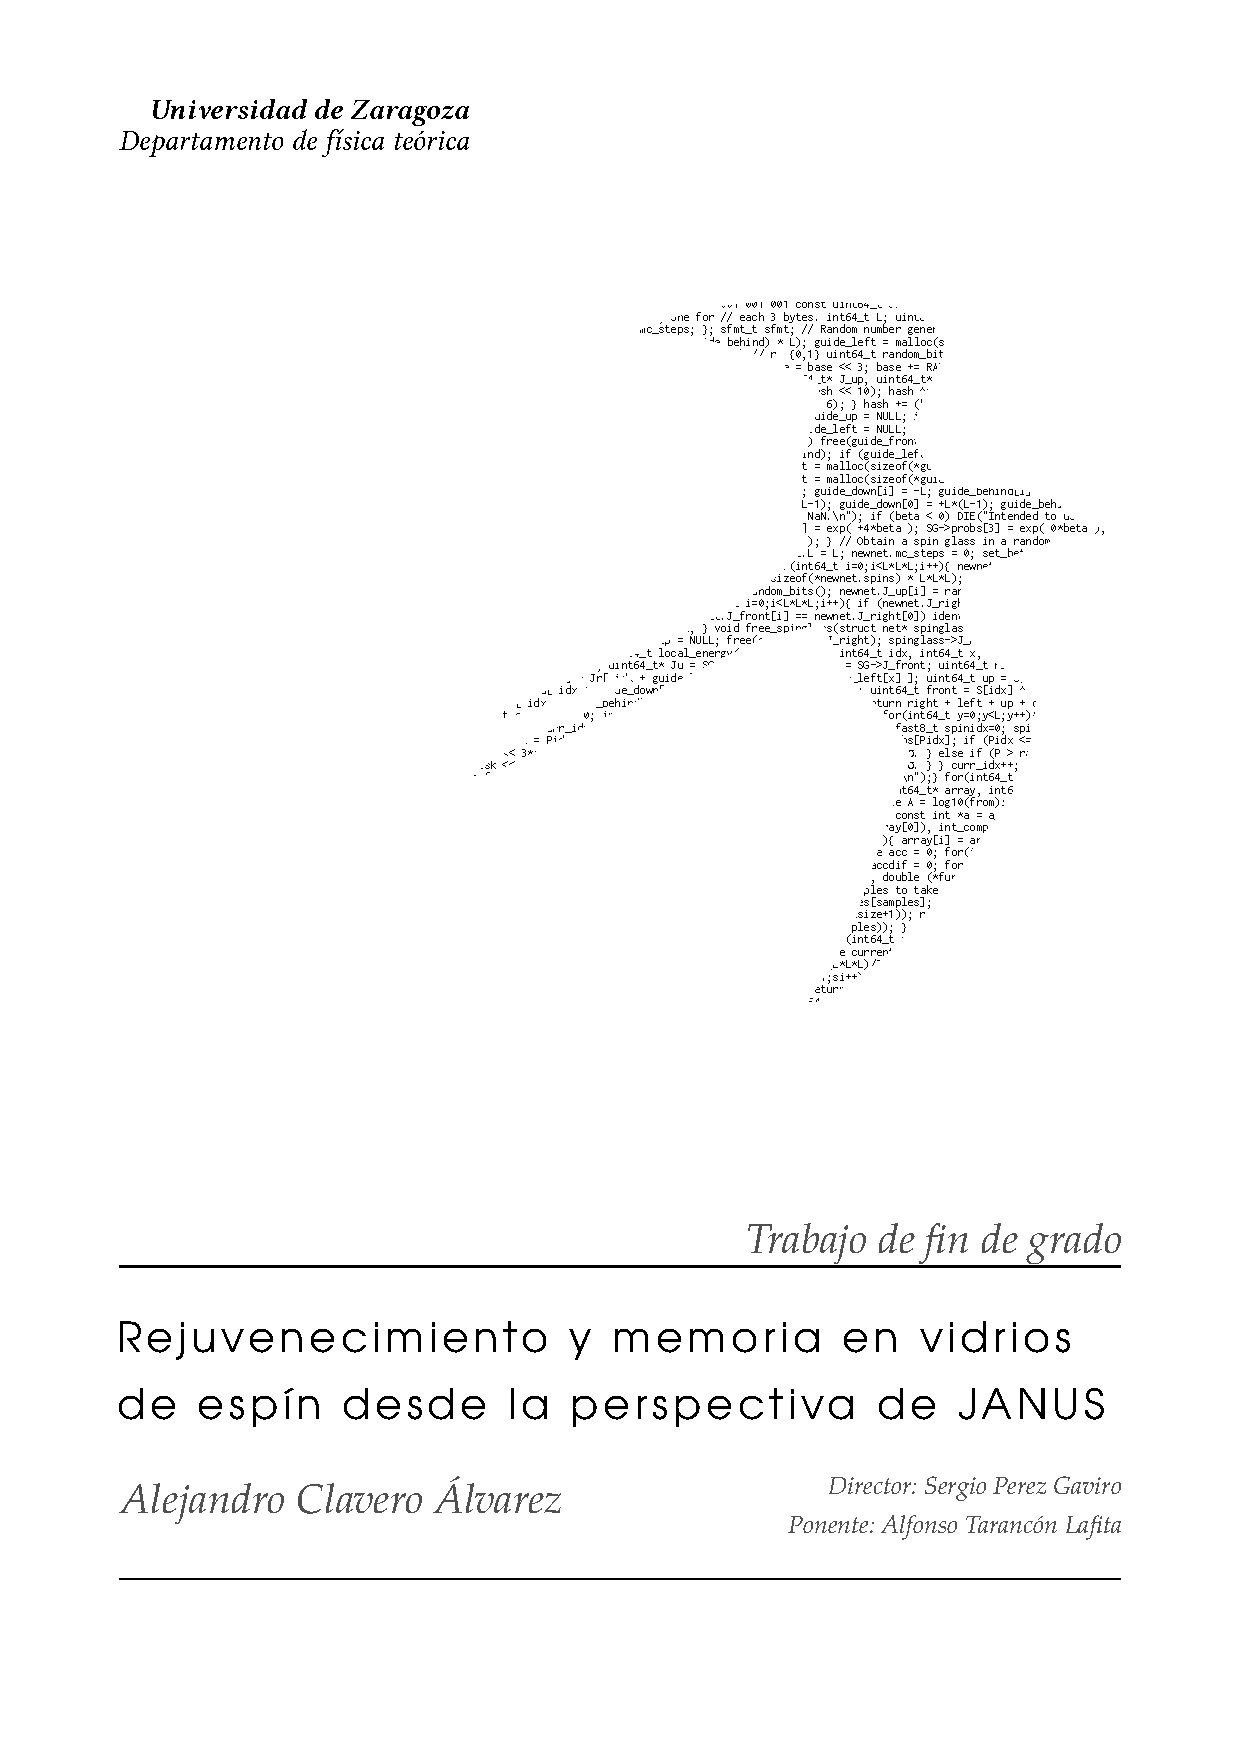
\includepdf{images/tfg_cover.pdf}
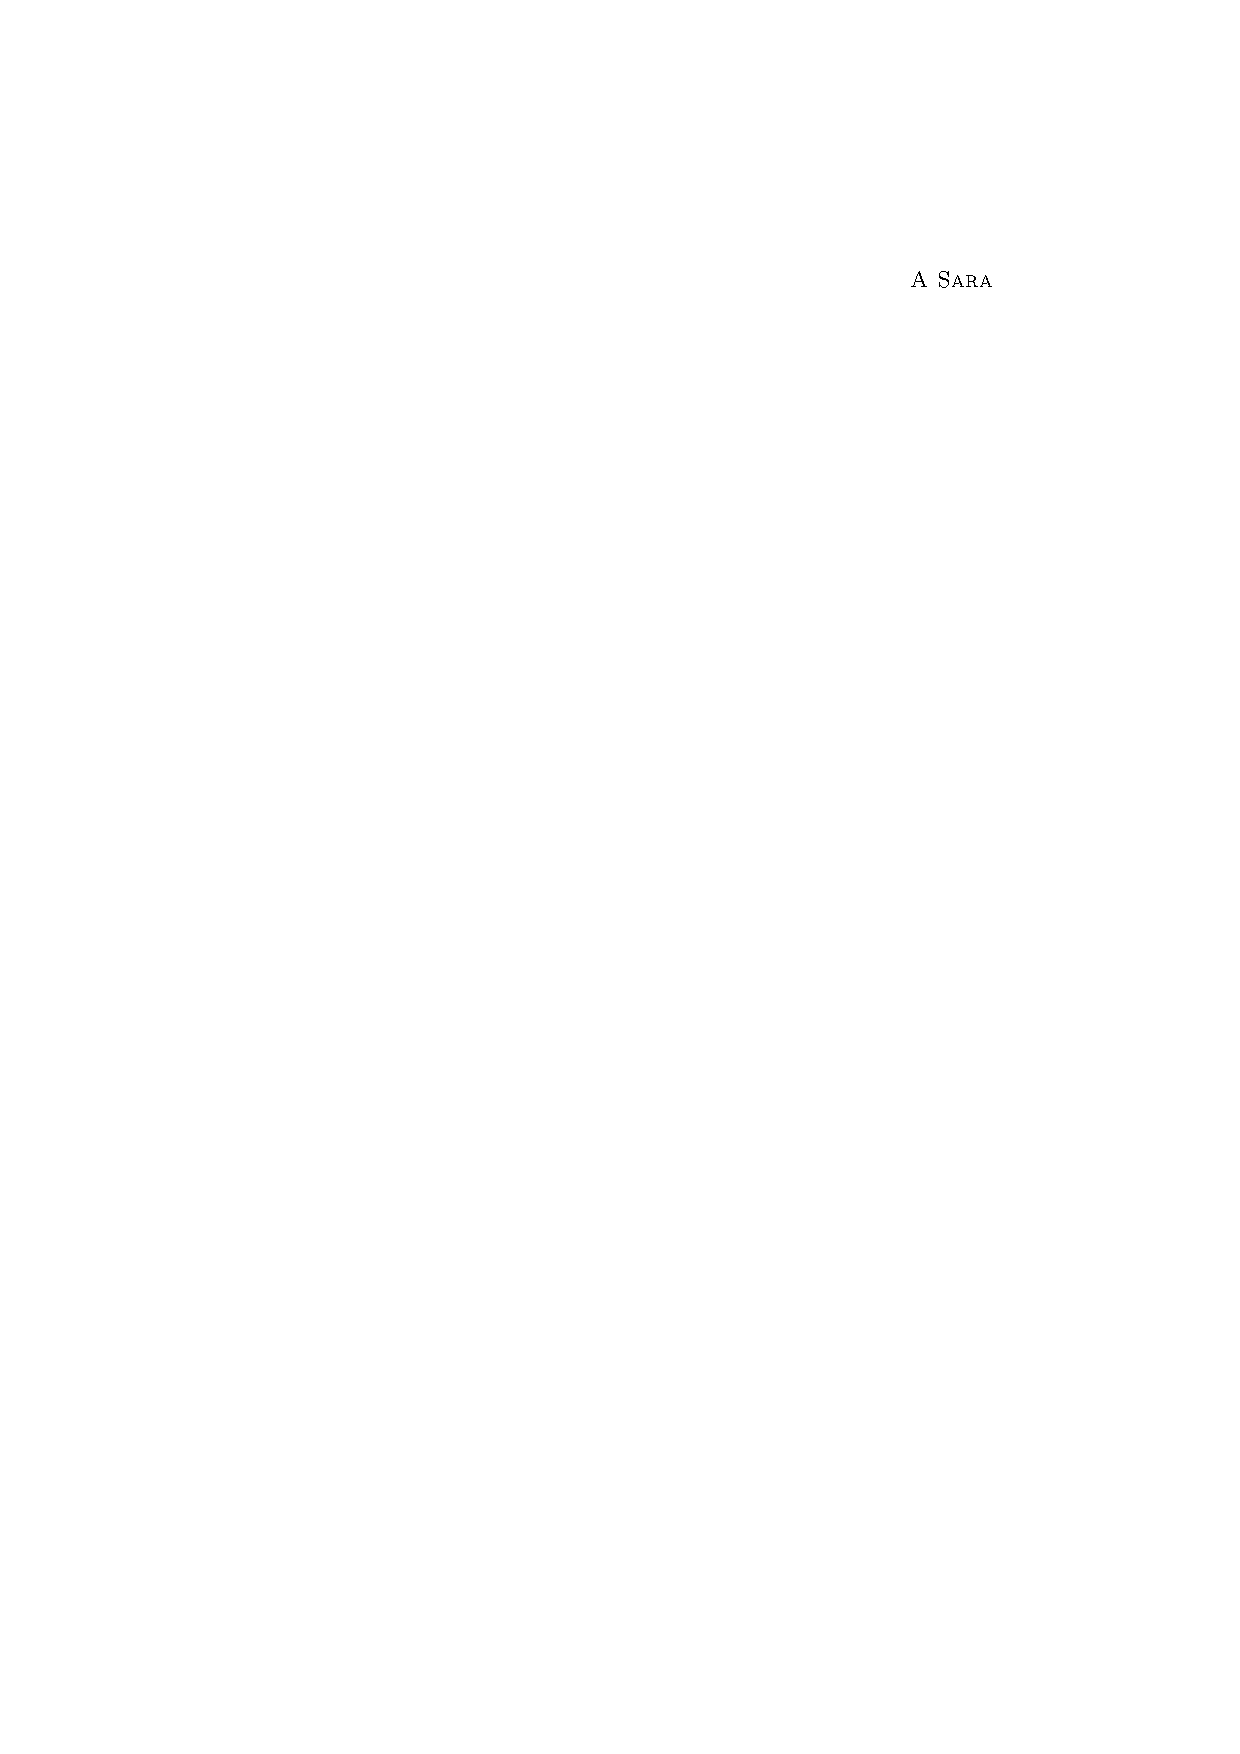
\includepdf{dedicatory.pdf}

\tableofcontents


\chapter{Introducción}

Los vidrios de espín
% TODO: REF 1
% Spin Glasses and Random Fields, edited by A. P. Young World
% Scientific, Singapore, 1997.
% TODO REF 2
% J. P. Bouchaud, L. Cugliandolo, J. Kurchan, and M. Mézard, in Spin
% Glasses and Random Fields
(\textit{spin glasses}) son materiales
caracterizados por el inusual comportamiento de sus momentos
magnéticos. En lugar de mostrar un alineamiento regular de éstos, como
los materiales ferromagnéticos o los antiferromagnéticos, los momentos
están distribuidos de forma aleatoria, de forma análoga a como la red
atómica de un vidrio está dispuesta de forma irregular frente a la
estructura regular de un cristal.

Por debajo de una temperatura crítica $T\sub{C}$ estos
materiales abandonan la fase paramagnética para pasar a una fase
conocida como \emph{fase vidrio de espín}, en la cual se dan los
efectos que se estudian en esta memoria: la \emph{memoria} y el
\emph{rejuvenecimiento}. Para entender dichos efectos, es
especialmente ilustrativo considerar dos tipos de experimento
(figura~\ref{fig:experimental}).

En el \textit{dip experiment protocol}~\cite{dippaper} se mide la
parte imaginaria de la susceptibilidad magnética $χ''=χ \sin φ$, donde
$φ$ es el desfase entre el campo $H$ aplicado y la magnetización $M$
de la muestra. La medición, que depende de la temperatura, se realiza
de la siguiente manera:

En primer lugar, recorremos el rango de temperaturas enfriando o
calentando el sistema a un ritmo constante, obteniendo la curva de
referencia. En segundo lugar, medimos enfriando el sistema a un ratio
determinado, pero cesando el enfriamiento durante un tiempo a una
temperatura elegida (en el caso mostrado, $T=\SI{12}{\K}$) y
retomándolo después; durante el tiempo que se deja reposar al sistema
a temperatura constante $χ''$ decae, efecto conocido como
envejecimiento. Por último, volvemos a medir $χ''(T)$ esta vez
calentando el sistema al mismo ratio y sin detenernos en
$T=\SI{12}{\K}$. Sorprendentemente, el sistema ``recuerda'' (efecto de
memoria) que su enfriamiento se cesó a $T=\SI{12}{\K}$ y en lugar de
seguir la curva de referencia medida sigue la de enfriamiento anterior,
volviendo a decrecer su susceptibilidad en $T=\SI{12}{\K}$ la misma
cantidad que decreció en el enfriamiento.

En el protocolo de dos temperaturas~\cite{threeprotocolpaper}
comenzamos con un vidrio de espín a temperatura $T_1=\SI{12}{\K}$.
Dejamos evolucionar al sistema a temperatura constante, y vemos que la
parte imaginaria de la susceptibilidad $χ''$ decae de forma continua,
efecto al que llamamos envejecimiento. A continuación, cambiamos a una
temperatura más baja $T_2=\SI{9}{\K}$. $χ''$ experimenta un
crecimiento súbito, efecto al que en contraposición con el
envejecimiento se le llama rejuvenecimiento. Por último, tras dejar
decrecer a $χ''$ por un tiempo a $T_2$, volvemos a calentar al sistema
a $T_1$. El sistema recupera de forma rápida la $χ''$ que tenía cuando
se pasó de $T_1$ a $T_2$, y continúa la evolución como si nunca
hubiera existido la fase a $T_2$, con la misma pendiente.


\begin{figure}
  \centering

  \makebox[1.2\linewidth]{
    \hspace*{-4cm}
    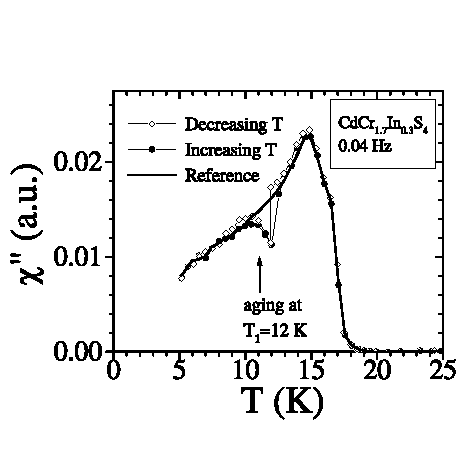
\includegraphics{./images/dip.pdf}
    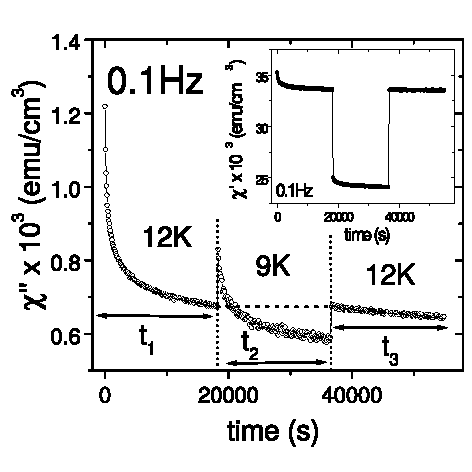
\includegraphics{./images/threetempsprotocol.pdf}
    }

    \caption{Experimentos que muestran los efectos de memoria y
      rejuvenecimiento en un vidrio de espín de
      CdCr\textsubscript{1.7}In\textsubscript{0.3}S\textsubscript{4}
      para la parte imaginaria $χ''$ y real $χ'$ de la
      susceptibilidad. En la figura izquierda (tomada de la figura 1
      de~\cite{dippaper}) vemos el \textit{dip experiment protocol} y en la
      derecha (tomada de la figura 1 de~\cite{threeprotocolpaper})
      el protocolo de dos temperaturas.}
  \label{fig:experimental}
\end{figure}

\section{Modelo}
Los primeros vidrios de espín~\cite{canella} que se estudiaron en los
años 70 consistían en metales nobles impurificados con metales de
transición, como por ejemplo el CuMn. Las impurezas crean perturbaciones aleatorias en la
red cristalina modelables mediante el \emph{modelo RKKY}, que propone
una interacción entre dos momentos magnéticos a distancia $r$ de la forma
\begin{equation}
  J(r) ∝ \frac{\cos(2K\sub{F} r)}{r^3}
\end{equation}
donde $K\sub{F} ∼ \SI{1e10}{\per\metre}$ es el vector de ondas del
metal impurificado. La función $J(r)$ tiene una oscilación debida al
término coseno de longitud de onda muy corta, cambiando de signo a
escala atómica.

Los momentos magnéticos de los vidrios de espín se modelarán mediante
espines discretos situados en una malla tridimensional de $L$ espines
de lado con espaciado regular, como propusieron Edwards y
Anderson~\cite{mranderson}. Supondremos únicamente interacciones a
primeros vecinos (figura~\ref{fig:EA}) y condiciones de contorno
periódicas, de forma que cada espín $s_i$ interactúe con sus seis
vecinos $s_j$ más proximos mediante un hamiltoniano
\begin{figure}
  \centering
  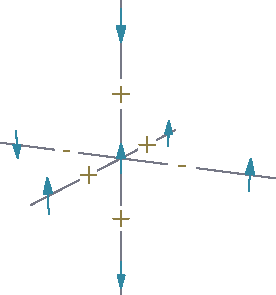
\includegraphics{../study_cases/EAfigure/EAfigure.pdf}
  \caption{Modelo de Edwards-Anderson en 3D, con interacciones a
    primeros vecinos. Cada espín interacciona únicamente con los 6
    espines más cercanos en la red, siendo el signo de la interacción
    aleatorio.}
  \label{fig:EA}
\end{figure}
\begin{equation}
  \Ham = - \sum_{\expval{i,j}}  J_{ij} s_i s_j
\end{equation}
donde los acoplos $J_{ij}∈\pm1$ de los espines $s_i∈\pm1$ son
números aleatorios de distribución plana, modelizando la rápida
variación de $J$ debida a la interacción RKKY. La función de
partición del sistema queda como
\begin{equation}
  \mathcal{Z} = [Z_J]
\end{equation}
donde ``$[\ ]$'' indica un promedio sobre sistemas con diferentes
acoplos $J_{ij}$, a los que llamaremos \textit{muestras}. Este
promediado esta justificado por las escalas de tiempos existentes en
el problema: los espines $s_i$ tienen una evolución mucho más rápida
que los acoplos, de forma los acoplos se pueden suponer fijos durante
las iteraciones que se pueden realizar en la simulación de los
sistemas. Los promedios usuales sobre el espacio de configuraciones de
una sola muestra se denotan como ``$\expval{\ }$''.


\section{Magnitudes}

Para estudiar la memoria y el rejuvenecimiento, se definieron y
midieron diversos observables del sistema. Es especialmente
interesante el comportamiento de estas magnitudes en el protocolo
de dos temperaturas al que se someterá a los vidrios de espín,
\begin{equation*}
  T_1 → T_2 → T_1
\end{equation*}
donde $T_2<T_1<T\sub{C}$ y los cambios de $T_1$ a $T_2$ y de $T_2$ a
$T_1$ se producen en $t_w^1$ y $t_w^2$ respectivamente.

La energía, de forma similar al hamiltoniano del sistema, se define como
\begin{equation}
  E = - \frac{1}{V} \sum_{\expval{i,j}}  J_{ij} s_i s_j
\end{equation}
con $V=L^{-3}$ y tomando valores entre $-1$ y $1$, es indispensable
para actualizar los espines en cada iteración del algoritmo de
Metropolis-Hasting~\cite{metropolis}. Tiene un comportamiento suave,
lo que la hace útil para comprobar si la simulación ha transcurrido de
forma normal, los datos no se han corrompido al guardarlos, etc.

En los sistemas ferromagnéticos es de especial interés la
magnetización del sistema, aquí definida como
$\frac{1}{V}\sum_{i}σ_i$, por ser el parámetro de orden. No obstante,
en los vidrios de espín los espines se congelan por debajo de
$T\sub{C}$ con magnetización global es nula~\cite{binder}, de forma
que es necesario definir como parámetro de orden el \textit{overlap}
entre los espines $s^a_i, s_i^b$ de dos réplicas a y b como
\begin{equation}
  q = \frac{1}{V} \sum_{i} s^a_i s_i^b
\end{equation}
donde se define como pareja de réplicas a dos sistemas con los mismos
acoplos $J_{ij}$ pero que han evolucionado de forma independiente, con
distintos números aleatorios en el proceso. Es una magnitud
comprendida entre $-1$ y $1$, cuyo valor en las simulaciones fluctúa
alrededor de $q=0$ con media nula, como puede verse más adelante en la
figura~\ref{fig:overlap}. La distribución del \textit{overlap} es
objeto de debate, habiéndose propuesto diferentes teorías a lo largo
de la historia de los vidrios de espín; las dos principales teorías en
las que se trabaja en la actualidad son la teoría
RSB~\cite{Marinari2000}\cite{mezard1987spin}, de las siglas inglesas
\textit{replica simmetry breaking}, y la \textit{droplet
  picture}~\cite{cmonman}.

La teoría \textit{RSB} propone un número infinito de estados en
equilibrio, de forma que la distribución $P(q)$ del \textit{overlap}
es no trivial y posee un continuo de estados entre dos máximos
simétricos. En cambio, en el \textit{droplet scenario} solo existe un
estado fundamental (salvo por una inversión de todos los espines) y
$P(q)$ consiste en dos deltas de Dirac.

La correlación a dos tiempos $t_w, t_w+t_0$ se define como
\begin{equation}
  C(t_w,t_w+t_0) = \frac{1}{V} \sum_{i}\expval{s_i(t_w)\ s_i
    (t_w+t_0)}
\end{equation}
donde $s_i∈$ son los $V$ espines del sistema. El parámetro $t_0$ está
relacionado con la frecuencia experimental de medición de la
susceptibilidad $ω$ como $t_0 ≃ 2π/ω$.

La magnitud en la que se ven con mayor claridad los efectos de memoria
y rejuvenecimiento es la susceptibilidad $χ$, que se puede calcular
gracias al teorema de fluctuación-disipación a través de la
correlación como
\begin{equation}
  χ(t_w, t_w+t_0) = β(1-C)
\end{equation}
donde $β=1/\kb T$ . Si bien este resultado solo es válido en
equilibrio térmico, condición extremadamente difícil de alcanzar en
sistemas con alta frustración como los vidrios de espín, se puede
extender fácilmente fuera de él multiplicando por una función $X$ que
solo depende de los tiempos $t_1,t_2$ empleados en la correlación. En
este trabajo, no se ha realizado dicha corrección por estar fuera de
los objetivos fijados y requerir un análisis más profundo de estos
sistemas.

Por último, mediante el \textit{overlap} se puede definir la
correlación espacial $C_4$ como
\begin{equation}
  C_4(r,t_w) =  \sum_{i} \expval{q_i(t_w)\ q_{i+r}(t_w)}
\end{equation}
donde $q_{i+r}$ es el \textit{overlap} del espín que está a distancia
$r$ del $i$. La magnitud, con valores entre $-1$ y $1$, aumenta
conforme el sistema se acerca al equilibrio ($t_w→∞$) y disminuye con
la distancia entre espines $r$.

\chapter{Objetivos}
El principal objetivo del trabajo presentado es caracterizar los
efectos de memoria y rejuvenecimiento en vidrios de espín. Para ello
ha sido necesario familiarizarse con los vidrios de espín, paradigma
de los sistemas complejos, y paralelamente realizar una inmersión a
fondo en la supercomputación, utilizando diferentes arquitecturas (PC,
\textit{clusters}, y ordenadores de propósito específico) y lenguajes
de programación (Python, C99, Julia~\cite{julialang} y Unix Shell)
con los que crear código que realizara y analizara las simulaciones.

Definiendo la energía de los estados como el valor del hamiltoniano se
puede explorar el espacio de configuraciones\footnote{ Temperaturas
  demasiado bajas no son explorables con este método. Valores muy
  altos para $β=1/\kb T$ crean un \textit{underflow} en el cálculo de
  $\exp(-βE)$, es decir, el procesador no puede distinguir $\exp(-βE)$
  de cero. No obstante, se ha comprobado que el límite está en
  $T=1/60$, muy inferior a las temperaturas usadas. }, y asignándoles
probabilidades $e^{-β \Ham}$ con $β=1/\kb T$ \  las magnitudes del
sistema introducidas pueden aproximarse mediante un algoritmo como el
de Metrópolis-Hasting~\cite{metropolis}: es simple de implementar,
acerca al sistema a la termalización antes que otros algoritmos como
el \textit{Heat bath} y es muy eficiente computacionalmente. El
algoritmo requiere una gran cantidad de números aleatorios, cuya
calidad se comprobó exhaustivamente (Apéndice \ref{chap:random}). Cada
iteración del algoritmo equivale a aproximadamente un picosegundo de
evolución en un experimento~\cite{tiempos}, lo que limita los
intervalos temporales en el estudio de estos sistemas a las décimas de
segundo.

Los cálculos se realizaron en el \textit{cluster} Memento y en el
ordenador de propósito específico Janus~\cite{janus}, basado en
FPGAs\footnote{Un FPGA (del inglés \textit{Field Programable Gate
    Array}) es un dispositivo basado en puertas lógicas que permite
  programar las conexiones entre sus puertas internas mediante un
  ordenador. Esto permite crear circuitos electrónicos adaptados a la
  aplicación, consiguiendo altas velocidades de cálculo.}. Para
calcular los observables es necesario un gran número de
muestras, lo que se consiguió de forma diferente en cada arquitectura:
\begin{itemize}
\item En el \textit{cluster} el gran número de nodos de computación,
  los múltiples hilos de ejecución por cada procesador, y el
  \textit{multispin coding}~\cite{onetruemultispincoding}
  (Apéndice~\ref{chap:multispin}) permiten simular miles de muestras
  simultáneamente.
\item En Janus, solo se ha podido simular del orden de una centena de
  vidrios de espín simultáneamente. No obstante, se utilizó para retículos
  grandes ($L>40$), en los que los efectos de tamaño finito son mucho
  menos notables y las fluctuaciones de los observables son menores,
  requiriendo promedios entre muchas menos muestras (decenas) para
  conseguir la misma incertidumbre en las medidas.
\end{itemize}
Para simulaciones de tiempos cortos y retículos pequeños que no
requirieron la potencia de cálculo de Memento y Janus se empleó un PC
doméstico.

Se decidió realizar todas las simulaciones bajo un protocolo
de dos temperaturas como el de la figura \ref{fig:experimental}:
\begin{enumerate}
\item El sistema, de un $L$ determinado, se deja evolucionar $t_w^1$
  pasos de Montecarlo a una temperatura $T_1$.
\item Una vez realizados los $t_w^1$ pasos de Montecarlo, se enfría de
  forma instantánea a $T_2<T_1$. En este cambio se medirá el efecto
  del rejuvenecimiento. El sistema permanece a $T_2$ hasta
  que se alcance el paso de Montecarlo $t_w^2$.
\item Alcanzado dicho paso, se vuelve a calentar instantáneamente el
  sistema a $T_1$. Se le deja permanecer a esta temperatura $10^8$
  iteraciones para poder observar la memoria del sistema.
\end{enumerate}
Además, se realizó una simulación de referencia a $T=T_1=\text{cte.}$
con la que comparar la susceptibilidad para medir rejuvenecimiento y memoria.

En dicho protocolo, se simuló
$t_w^1 ∈\{10^4, 10^5, 10^6, 10^7, 10^8\}$,
$T_1∈\{0.9, 0.8, 0.7, 0.6\}$, $T_2∈\{0.8,0.7.0.6\}$ y se empleó
$t_0∈\{10^4, 10^5, 10^6, 10^7,10^8\}$. Hay que notar que las $t_0 ≫
t_w$ no son accesibles experimentalmente, pero por completitud se
incluyeron en el análisis.

Se emplearon varios tamaños $L$
de retículo para la simulación de referencia, $L∈\{4,6,8,12\}$ en
Memento y $L∈\{8,48,80\}$ en Janus. El protocolo de dos temperaturas
pudo completarse hasta $t_w^2$ para $L∈\{8,12,48,80\}$ y más allá para
$L∈\{8,48,80\}$.
Como valor para $t_w^2$, se escogió $t_w^1 + 10^8$ para las redes de
Memento y $2×10^8$ para las redes de Janus.

Más adelante se definirán magnitudes escalares que permitan
cuantificar la memoria y el rejuvenecimiento con objeto de realizar un
análisis de sus dependencias funcionales con $t_w^1$, $t_0$ y
$\frac{T_1-T_2}{T_1}$.


\chapter{Desarrollo}

Los tiempos de simulación y medición de magnitudes llegan a la semana
para algunos tamaños del sistema, por lo que es imprescindible una
buena organización a la hora de programar las simulaciones y las
medidas. Además, es importante comprobar que los sistemas están
evolucionando como se espera, sin fallos de \textit{software} o
\textit{hardware} que invaliden los resultados. Por ello, mientras se
obtenían las configuraciones de espines se comprobó que todos los
observables del sistema tenían el comportamiento esperado, como se
verá a continuación.

\section{Comportamiento de los observables}

Un observable especialmente útil para comprobar que no ha habido
fallos graves en la simulación es la energía, que ha de tener un
comportamiento suave y continuo como el que muestra la figura
\ref{fig:energyprotocol}. El \textit{overlap}, como muestra la figura
\ref{fig:overlap}, debe tener un histograma centrado en cero y una
distribución de doble pico simétrica.

\begin{figure}
  \centering
  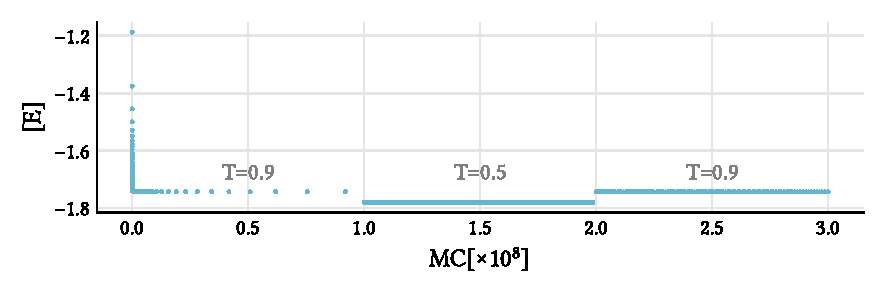
\includegraphics{../study_cases/energy_in_protocol/energyprotocol.pdf}
  \caption{Energía para un sistema $L=80$ promediada sobre 8 muestras.}
  \label{fig:energyprotocol}
\end{figure}

\begin{figure}
  \centering
  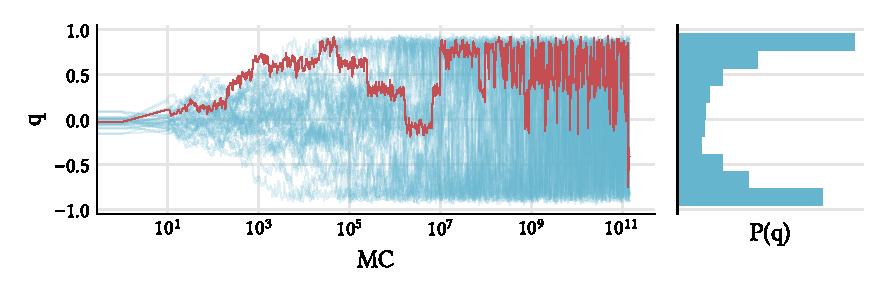
\includegraphics{../study_cases/overlap/overlap.pdf}
  \caption{Fluctuaciones del overlap $q$ para $L=8$, uno de los pocos
    tamaños que puede llevarse hasta $10^{11}$ iteraciones de
    Montecarlo en un tiempo de días. Se muestran en el fondo (azul) el
    overlap de 32 muestras y en rojo el de una de ellas. A la derecha
    se muestra un histograma de la distribución del overlap de las
    muestras por encima de $10^8$ pasos de Montecarlo.}
  \label{fig:overlap}
\end{figure}

Como puede verse en la figura~\ref{fig:corrfunction}, los sistemas
están más descorrelacionados cuanto más aumentamos el intervalo
temporal $t_0$ debido a que se comparan configuraciones de espines
separadas por un mayor tiempo, y van alcanzando un estado global de
mayor correlación conforme lo dejamos evolucionar ($t_w → ∞$) y el
sistema se acerca lentamente al equilibrio térmico.

\begin{figure}
  \centering
  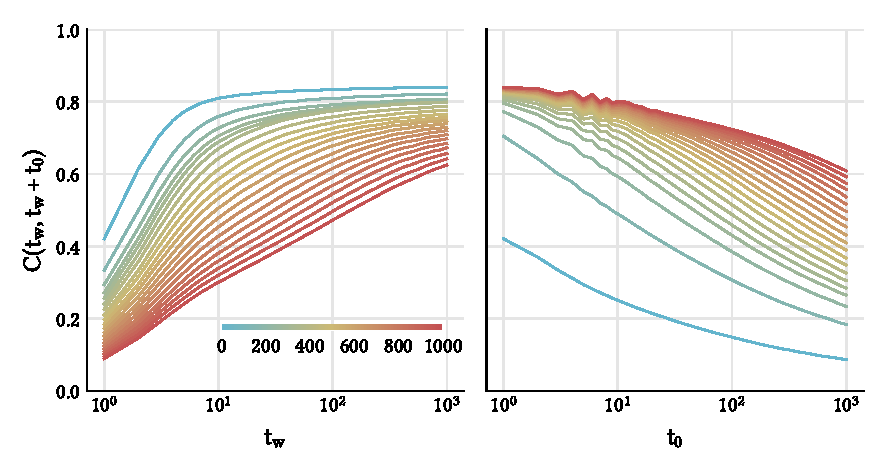
\includegraphics{../study_cases/corr_functional_dependence/corrfunction.pdf}
  \caption{Correlación para un sistema $L=32$ promediada sobre 210
    muestras. Se muestra en la escala de color el parámetro ($t_0$ o
    $t_w$) no empleado en el eje horizontal. Ambos parámetros toman
    valores $t_0,t_w∈[1, 10^3]$.}
  \label{fig:corrfunction}
\end{figure}

La dependencia de la correlación con $L$ es mucho más marcada para
$t_0$ elevado, como puede verse en la figura~\ref{fig:corrfunction_L}.
También vemos que de forma cualitativa la correlación crece
monótonamente con $L$ para $t_w→∞$.

\begin{figure}
  \centering
  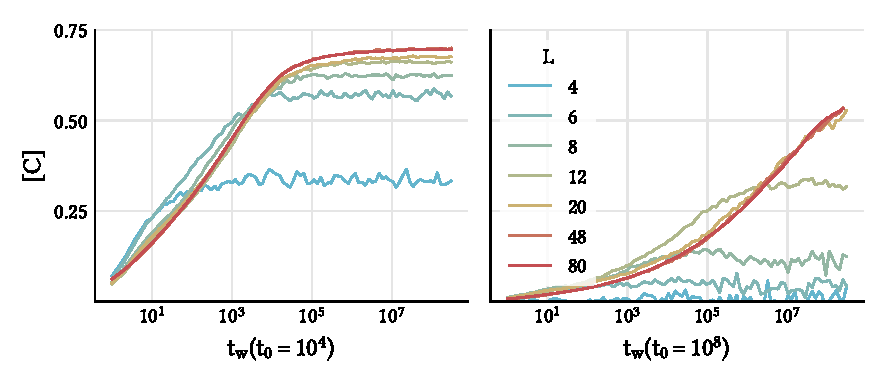
\includegraphics{../study_cases/correlation_L_dependence/corrwithL.pdf}
  \caption{Correlación a $T=0.9$ promediada sobre más de 1000 muestras
    para $L<40$ y sobre más de 30 para $L>20$ (color en el original).
    Para $t_0$ y $t_w$ bajos, las medidas de la correlación están menos
    afectadas por la $L$ del sistema.}
  \label{fig:corrfunction_L}
\end{figure}


La correlación espacial es especialmente interesante para
saber si la muestra va a mostrar unos efectos de tamaño finito
fuertes, ya que con ella se puede hallar la longitud de correlación
$ξ$ mediante el ajuste asintótico~\cite{c4fit}
\begin{equation}
  C_4 (r,t_w) \stackrel{L→∞}{=} \frac{A}{r^α} \exp \left( [-r/ξ(t_w)]^β \right)
  \label{eq:fitotron}
\end{equation}
o mediante integración~\cite{c4integration} de $C_4$ con
\begin{equation}
  ξ(t_w) ≃ \frac{\int_0^{L/2} r^2 C_4(r, t_w) \dd{r}}{\int_0^{L/2} r C_4(r, t_w) \dd{r}}
  \label{eq:integranator}
\end{equation}

Nótese que no tiene sentido ver el valor de $C_4$ para $r>L/2$, ya que
las condiciones de contorno periódicas implican que la distancia entre
dos espines es siempre igual o menor que ese valor. Una longitud de
correlación cercana a este valor es señal de que el retículo es
demasiado pequeño como para tenerlo en cuenta.

Se consideró cuál de los métodos para hallar $ξ$ emplear; en la
figura~\ref{fig:c4} se puede ver un ejemplo de los resultados de ambos
para un retículo con $L=12$. Se escogió el método mediante integrales
de la ecuación \eqref{eq:integranator} por ser mucho más preciso para
$t_w≫10^7$ que el ajuste a la ecuación~\ref{eq:fitotron}~\cite{c4integration}.

En la figura~\ref{fig:C4_with_size} se muestran los resultados
obtenidos para la longitud de correlación. Como se puede ver, siempre se
tiene $ξ ≪ L/2$, tal y como se buscaba.


\begin{figure}[!h]
  \centering
  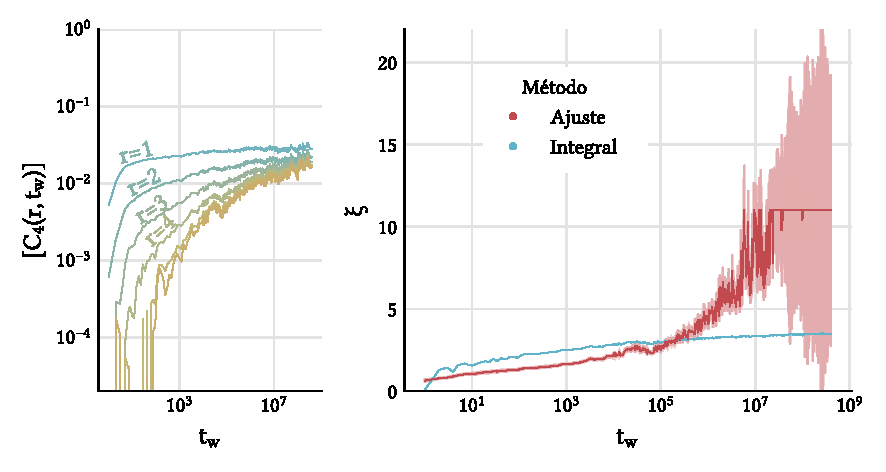
\includegraphics{../study_cases/c4_functional_dependence/C4_handedit.pdf}
  \caption{En la figura izquierda se muestran los valores de $C_4$
    medidos para un retículo $L=12$ a $T=0.9$, correspondiendo cada
    línea a un $r∈\{1,2,\ldots,6\}$ junto a los $ξ$ obtenidos mediante
    el ajuste y mediante integración en la figura derecha (color en el
    original). Para $t_w$ alta el ajuste de $C_4$ es malo y la
    incertidumbre (zona sombreada) crece sin límite.}
  \label{fig:c4}
\end{figure}

\begin{figure}[!h]
  \centering

  \vspace{1cm}

  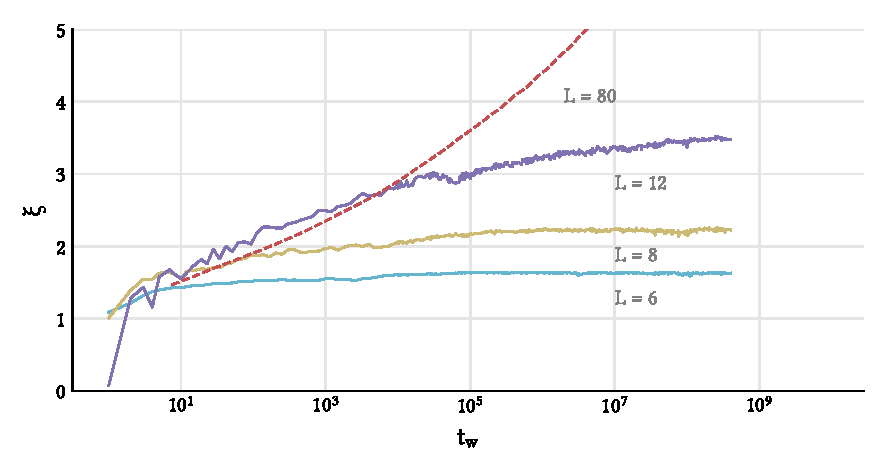
\includegraphics{../study_cases/c4_functional_dependence/C4_with_size.pdf}
  \caption{La longitud de correlación $ξ$ a $T=0.7$ es menor que $L/2$
    en todo el rango de $t_w$ empleado; la imagen no cambia
    sustancialmente para otras temperaturas $T<T\sub{C}$. Los datos
    para $L=80$ se han extraído de \cite{c4integration}.}
  \label{fig:C4_with_size}
\end{figure}


\begin{figure}
  \centering
  \begin{tikzpicture}
    % Axis
    \draw[NiceBlack] (0,0) -- (10,0) node [below, NiceBlack] {$t_w$};
    \draw[NiceBlack] (0,0) -- (0,4) node [left, NiceBlack] {$χ$};
    % help lines
    \draw[thin, black!20!white] (3,2) -- (3,0);
    \draw[thin, black!20!white] (3.8,0.85) -- (3.8,0);
    \draw[thin, black!20!white] (3,2) -- (1.2,2);
    \draw[thin, black!20!white] (1.2,2) -- (1.2,0);
    % Curves
    \draw[ultra thick, PlotDefault] (0.5,4) to[out=-90, in=170] (3,1);
    \draw[ultra thick, dashed, PlotDefault!60!white] (3,1) to[out=-10,
    in=175] (6,0.6); % Extension
    \draw[ultra thick, PlotDefault] (6,1) to[out=-10, in=175] (9,0.6);
    \draw[ultra thick, PlotSecondary] (3,2) to[out=-85, in=180]
    (6,0.5);
    % measures
    \fill[gray] (1.2,0) circle (0.1) node[below, NiceBlack]
    {$t_\mathit{rej}^L$};
    \draw[<->, NiceBlack] (1.2,2) -- (3,2) node[midway, above,
    NiceBlack] {$Δt_\mathit{rej}^L$};
    \draw[<->, NiceBlack] (3.0,2) -- (3.0,1) node[midway, left,
    NiceBlack] {$Δχ$};
    \draw[<->, NiceBlack] (3,-0.2) -- (3.8,-0.2) node[midway, below,
    NiceBlack] {$t_\mathit{rej}^A$};
  \end{tikzpicture}
  \caption{Definiciones cuantitativas del rejuvenecimiento en un
    protocolo de dos temperaturas. Se muestra la susceptibilidad $χ(t_w)$.}
  \label{fig:definitions}
\end{figure}


\section{Rejuvenecimiento}
Antes de estudiar el rejuvenecimiento es importante encontrar una
definición cuantitativa; en la figura \ref{fig:definitions} se
exponen las posibles definiciones creadas para el protocolo
de dos temperaturas.

Hasta ahora solo se han visto ejemplos de rejuvenecimiento
\emph{fuerte}, en el que la susceptibilidad sube por encima del valor
que tenía en $T_1$ al cambiar a $T_2$. No obstante, en algunas de las
mediciones se detectó rejuvenecimiento \emph{débil}, en el que la
curva de $χ$ no sube por encima de $T_1$ al efectuar el cambio a
$T_2$. $Δχ$ es la única magnitud que no diverge en esos casos, por lo
que se usará en el análisis. Para el caso del rejuvenecimiento débil
tendrá valores negativos.

Se realizó un \textit{bootstrap}~\cite{boot}
(Apéndice~\ref{chap:bootstrap}) de $χ(t_w)$ de las muestras de forma
que se tuviera una incertidumbre para los $Δχ$ hallados, que se
calcularán restando la $χ$ de referencia a $T_1$ y la $χ$ de la fase a
$T_2$ en $t_w = t_w^1$. El número de muestras tomadas varía según los
parámetros $t$,  $t_w^1$ y $\frac{T_1-T_2}{T_1}$, pero se encuentra siempre
entre 15 y 30 para los retículos $L>40$ y es superior a mil para los
$L<40$. Además, por cada muestra se promediaron dos réplicas.


\section{Memoria}

Antes de analizar los datos tomados, se realizó una pequeña simulación
con $t_w$ bajo y gran cantidad de estadística para ver cómo se
manifestaba la memoria en un caso ideal (figura~\ref{fig:memorytoy}).
En ella se aprecia como existe un pequeño tiempo en el que el sistema
todavía no ha recuperado la curva de referencia. Podemos caracterizar
ese tiempo $Δt$ viendo cuántas iteraciones pasan hasta que ambas
curvas se cruzan, obteniéndose una magnitud escalar para la memoria.

\begin{figure}
  \centering
  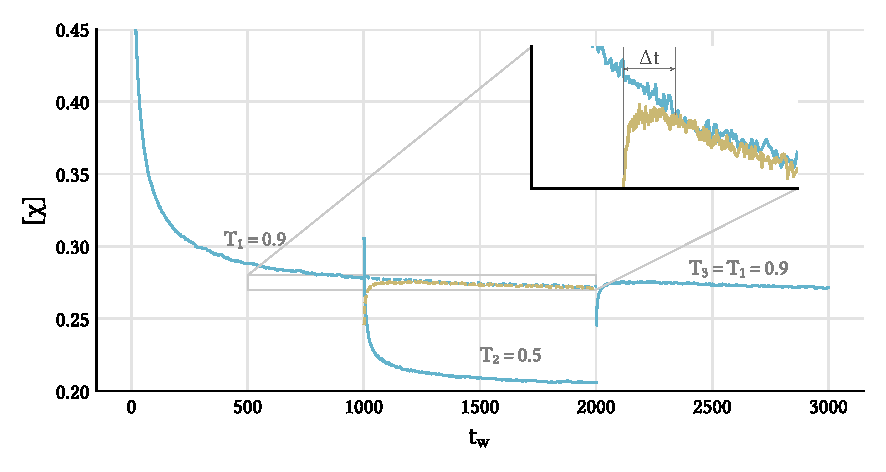
\includegraphics{../study_cases/memory_toy/memorytoy_handedit.pdf}
  \caption{Tras volver a $T_1$ desde $T_2$ el sistema (promedio sobre
    10500 muestras, $L=12$) recupera la curva $χ(T_1)$ desde donde se
    produjo el cambio a $T_2$. Se muestran en línea discontinua azul
    una simulación a $T_1$ sin cambio a $T_2$ como referencia, y en
    línea discontinua amarilla la curva para $T_3$ desplazada a la
    izquierda para facilitar la comparación.}
  \label{fig:memorytoy}
\end{figure}

\chapter{Resultados}
Una vez hallados los $Δχ$ en $t_w^1$ podemos analizar el efecto del
rejuvenecimiento, y con los $Δt$ hasta que el sistema recupera la
memoria podemos cuantificar ésta en función de los parámetros.

\section{Rejuvenecimiento}
Se comprobó si el parámetro $t_0$ de la correlación jugaba un papel
importante en la aparición de rejuvenecimiento débil. Como puede verse
en la figura~\ref{fig:vanishing}, en la que se realizó una simulación
para baja $t_w$, aumentar $t_0$ hace disminuir $Δχ$ de forma consistente
hasta que desaparece el rejuvenecimiento fuerte para
$t_0∼\frac{1}{2}t_w^1$. No obstante, hay que notar que experimentalmente
$ωt_w >1$, por lo que $t_0 < 2πt_w $, lo que restringe el rango de
$t_0$.

\begin{figure}
  \centering
  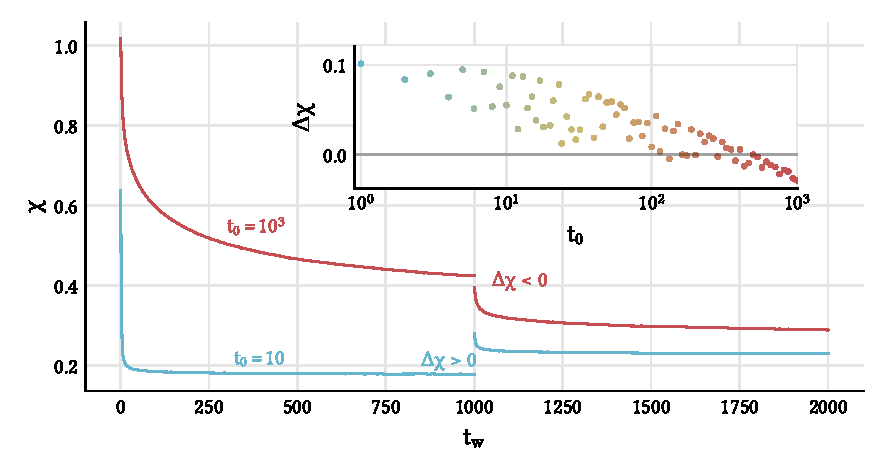
\includegraphics{../study_cases/vanishingrejuvenation/trej.pdf}
  \caption{Susceptibilidad $χ$ para $T_1=0.9, T_2=0.5, L=8$
    promediadas sobre $31500$ muestras con valores de $t_0∈[1,10^3]$,
    color en el original. El rejuvenecimiento fuerte desaparece cuando
    $t ≃ \frac{1}{2} 10^3$.}
  \label{fig:vanishing}
\end{figure}


En la figura~\ref{fig:trejanalysis}, puede verse que los parámetros de
los que depende el rejuvenecimiento ($t_w^1, t_0,
\frac{T_1-T_2}{T_1}$) tienen una influencia distinta sobre~$Δχ$.

Notamos que el valor de $Δχ$ parece tener un mínimo en $t_0$, visible
únicamente para $t_w^1 ≲10^5$. Además, hay un cambio en el
comportamiento de $Δχ$ conforme aumentamos $t_0$, que corresponde
experimentalmente a disminuir la frecuencia de medición de la
susceptibilidad: para $t_0$ bajo, una mayor $t_w^1$ implica un mayor
rejuvenecimiento $Δχ$, mientras que para $t_0$ alto (rango inaccesible
experimentalmente) ocurre al revés, y menores $t_w^1$ exhiben mayor
$Δχ$. Como predecía el pequeño experimento de la
figura~\ref{fig:vanishing}, las redes que muestran rejuvenecimiento
fuerte pasan a mostrar rejuvenecimiento débil al aumentar $t_0$.

La influencia de $T_1-T_2$ no es muy clara para $L>8$, pero para $L=8$
parece que aumentar dicha diferencia hace disminuir $Δχ$. En todo caso, es el
parámetro que menos influye en el rejuvenecimiento, probablemente por
ser el rango de valores tomados en el resto de parámetros mucho mayor.

Por último, notamos que solo se ha obtenido rejuvenecimiento fuerte
para $L=48$ y $L=80$, lo que indica que el tamaño de la red es
relevante en la aparición de este efecto.


\begin{figure*}
  \centering
  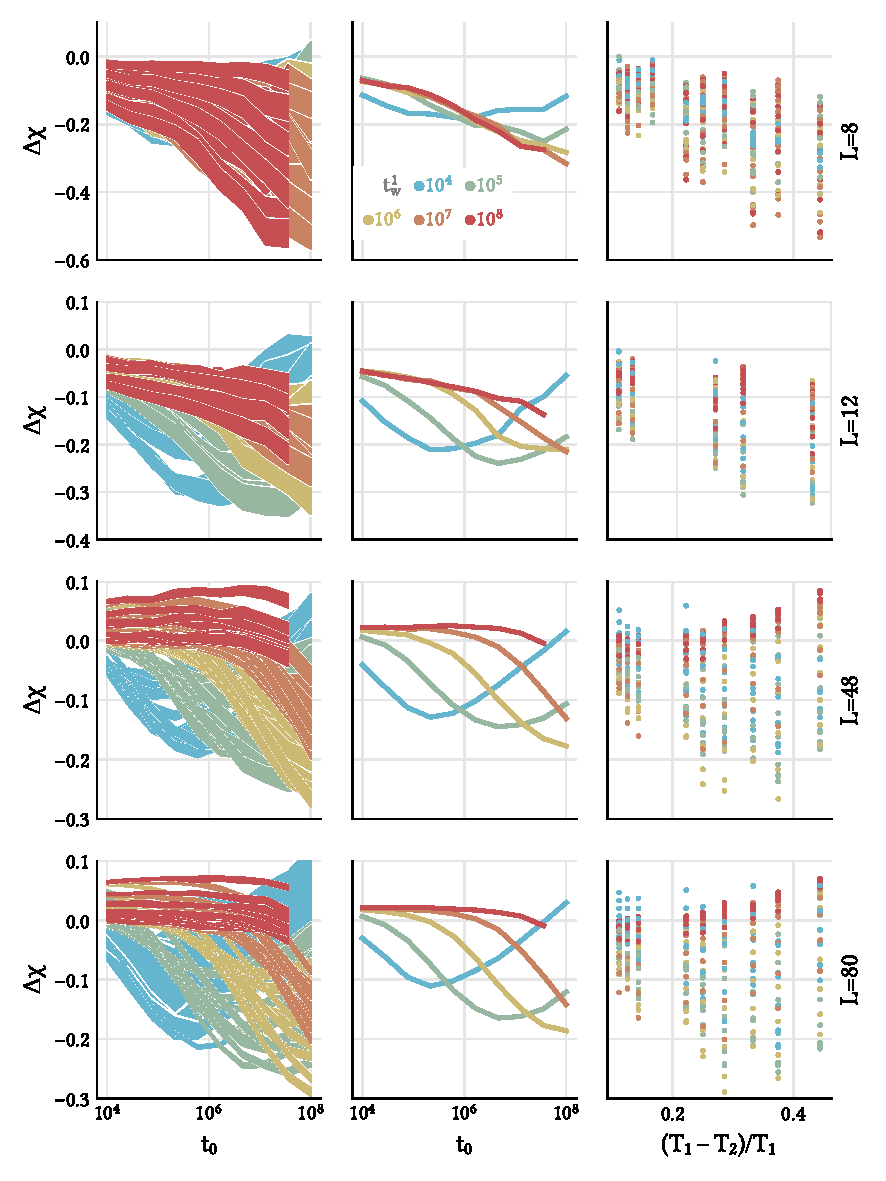
\includegraphics{../study_cases/trejanalysis/1D_dependence.pdf}
  \caption{En la columna izquierda se muestran bandas con las medidas
    de $Δχ$ tomadas para cada grupo de parámetros
    $(t_w^1, t_0, \frac{T_1-T_2}{T_1})$, correspondiendo el grosor a
    la incertidumbre a 1σ. En la columna central, se ven esas mismas
    medidas promediando sobre las distintas temperaturas medidas. A la
    derecha se muestra el valor medio del $Δχ$ según la relación entre
    las temperaturas $T_2$ y $T_1$, de nuevo para todos los grupos de
    parámetros medidos. En color se indica $t_w^1$, como muestra la
    leyenda.}
  \label{fig:trejanalysis}
\end{figure*}


\section{Memoria}

Para explorar la forma funcional de $Δt$, se optó por representarlo en
función de $t_w^1$, $t_0$ o $\frac{T_2-T_1}{T_1}$
y promediar sobre el resto, de forma que pudieran verse tendencias
generales (figura~\ref{fig:memdep}). Analizando los resultados, vemos
que $Δt$ crece con $t_0$ y disminuye con $t_w^1$ y con la diferencia
de temperaturas $T_1, T_2$. Notamos que el comportamiento del retículo
$L=8$ es anómalo respecto al de las redes $L=48$ y $L=80$,
probablemente por su pequeño tamaño. Para $t_w^1 > 10^6$, éste llega a
mostrar un rejuvenecimiento inmediato, alcanzando la curva de
referencia en una sola iteración de Montecarlo. Además, los tiempos de
recuperación $Δt$ son notablemente más pequeños para el retículo
$L=8$, cinco órdenes de magnitud menores que $L=48$ y $L=80$. Esto es
achacable a que su evolución es notablemente más rápida.

\begin{figure}
  \centering
  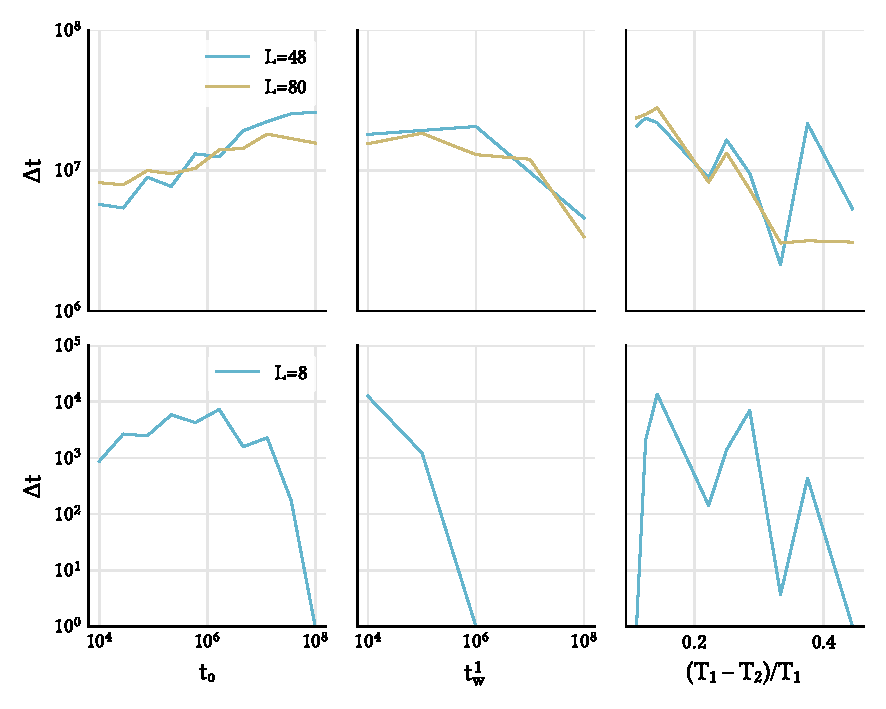
\includegraphics{../study_cases/memory/dependences.pdf}
  \caption{Se muestra el tiempo $Δt$ necesario para que el sistema
    recupere la curva de referencia tras volver a $T_1$ en función de
    $t_0$,$t_w^1$ o $\frac{T_1-T_2}{T_1}$ y promediando sobre el
    resto. Se indica en color el tamaño del sistema simulado.}
  \label{fig:memdep}
\end{figure}



\chapter{Conclusiones}
A lo largo del trabajo realizado se ha comprobado que la simulación de
vidrios de espín es un tema delicado y duro, requiriendo grandes
cantidades de tiempo tanto humano como de CPU. A pesar de la
simplicidad del modelo empleado, se ha visto como el comportamiento
del sistema era rico y variado.

A la hora de emplear tanto el \textit{cluster} como Janus, se tuvieron
diversos problemas técnicos que requirieron adaptar las simulaciones
numerosas veces para evitar la pérdida de datos. Las simulaciones de
vidrios de espín duran días, aumentando la probabilidad de aparición
de errores, especialmente en máquinas con varios años de uso como
Janus. Por ello, se realizaron distintos tests sobre el
\textit{software}, incluyendo la simulación de modelos de Ising, la
obtención de los valores medios de las ecuaciones de
Schwinger-Dyson~\cite{schwinger} y el ajuste de la correlación
$C(t_w,t_w+t_0)$ a una ley de potencias~\cite{corrparisi}.

En el estudio del rejuvenecimiento, se ha comprobado como el
rejuvenecimiento fuerte era especialmente frágil, mostrando la mayoría
de los datos tomados rejuvenecimiento débil. La frecuencia de medición
$ω$ de la susceptibilidad, a través del tiempo de correlación $t_0$,
juega un papel importante en el efecto junto al tiempo en que se
cambia la temperatura del sistema, $t_w^1$.

La memoria ha resultado ser un efecto mucho más robusto, aunque su
forma funcional no se haya conseguido analizar con la misma precisión
que el rejuvenecimiento. En esta magnitud es especialmente claro el
comportamiento anómalo de retículos pequeños ($L=8$), lo que justifica
la simulación de sistemas cada vez más grandes y la necesidad de
recursos computacionales cada vez más potentes.

Por último, me gustaría aprovechar estas líneas para dar las gracias
al BIFI por permitirme realizar parte de las simulaciones en sus
instalaciones y a la \textit{Janus Collaboration} por cederme tiempo
de cómputo en su máquina, Janus.

\begin{appendices}


\chapter{Bootstrapping}
\label{chap:bootstrap}
En ocasiones se quiere hallar el valor de un observable, pero no se
posee una magnitud que sea adecuado asociar con el error de la medida;
por ejemplo, la desviación estándar de una lista de valores no es un
estimador de la incertidumbre de su media. Esto se solucionó empleando
técnicas de remuestreo, concretamente
\textit{bootstraping} (remuestreo con reemplazamiento)~\cite{boot}.

Supongamos que tenemos una lista de $N$ valores $v_i$, y queremos hallar su
media. Si bien es trivial emplear $\frac{1}{N} \sum_{i=1}^N v_i$ para
ello, no conocemos cuál es la incertidumbre de dicha medición.

En un \textit{bootstraping}, se toman de forma aleatoria $M$
muestras con una fracción $f$ de los elementos originales. Si por
ejemplo $v = \{1,2,3,4,5,6,7,8,9\}$ y $f=\nicefrac{1}{3}$, empleando
$M=5$ obtenemos 5 listas de $9/3=3$ elementos.
Notar como el muestreo es con reemplazamiento, y por lo tanto puede
haber repeticiones. A continuación, calculamos el valor de la función
sobre cada muestra, obteniendo $M$ valores para la función, en este
caso la media:
\begin{equation*}
  1,2,3,4,5,7,8,9 \ \rightarrow \
  \begin{cases}
    5,5,2 \\
    8,1,7 \\
    1,9,5 \\
    7,7,4 \\
    3,9,7 \\
  \end{cases}
  \ \stackrel{\mathit{Media}}{→} \
  \begin{cases}
    4.0 \\
    5.3 \\
    5.0 \\
    6.0 \\
    6.3 \\
  \end{cases}
\end{equation*}
Por último, calculamos la media y la desviación estándar de los $M$
valores obtenidos, obteniendo así un estimador de la incertidumbre de
la función y su valor medio.

La elección del parámetro $M$ es fácil, ya que basta con que sea lo
suficientemente grande como para garantizar que todos los valores se
empleen. Como las listas sobre las que se realizó
\textit{bootstraping} en este trabajo tenían unos cien elementos, se
escogió $M=10^3$.
Como valor para el tamaño de los intervalos se
escogió una fracción $f = 1/e$ de los datos, como propone el
\textit{Numerical Recipes}~\cite{numericalrecipes}.

\chapter{Números aleatorios}
\label{chap:random}



\definecolor{PASSED}{HTML}{00693E}
\definecolor{WEAK}{HTML}{D2691E}
\definecolor{FAILED}{HTML}{B22222}


La elección del generador de números pseudoaleatorios es crucial para
realizar una simulación de Montecarlo, ya que puede sesgar
notablemente los resultados~\cite{randommonte}\cite{randomcoins} o
convertirse en el cuello de botella del programa si es muy lento.

A la hora de escoger un generador de números pseudoaleatorios, se primó la
correctitud en primer lugar y la velocidad en segundo. En la tabla
y gráfica siguiente pueden verse algunos de los resultados de la suite de tests
\verb|dieharder|~\cite{brown-2013}. Los tests son muy variados, pero a
modo de ejemplo se muestra la descripción que la propia suite de tests
provee para el test \verb|diehard craps|:

\begin{verbatim}
 This is the CRAPS TEST. It plays 200,000 games of craps, finds
 the number of wins and the number of throws necessary to end
 each game.  The number of wins should be (very close to) a
 normal with mean 200000p and variance 200000p(1-p), with
 p=244/495.  Throws necessary to complete the game can vary
 from 1 to infinity, but counts for all>21 are lumped with 21.
 A chi-square test is made on the no.-of-throws cell counts.
 Each 32-bit integer from the test file provides the value for
 the throw of a die, by floating to [0,1), multiplying by 6
 and taking 1 plus the integer part of the result.
\end{verbatim}

Si suponemos como hipótesis nula, $H_0$, que el generador de números
pseudoaleatorios sea indistinguible de uno realmente aleatorio,
podemos realizar diversos tests sobre los números y ver el
\textit{p-value} de la distribución obtenida conociendo la esperada
bajo números realmente aleatorios. Por ejemplo, si lanzamos una moneda
virtual, esperamos ver una distribución binomial, que podemos comparar
con la obtenida para hallar el \textit{p-value}.

Los propios \textit{p-values} están distribuídos de forma estadística,
así que esperamos ver fallar incluso a un generador perfecto un tanto
por ciento determinado de las veces. Esto hace que no solo haya que
rechazar generadores con un \textit{p-value} muy bajo, sino también
los que tengan un \textit{p-value} muy alto. La suite de tests, por
defecto, es conservadora y anuncia como ``débiles'' los tests con
$p>0.995$ y $p<0.05$ y como ``fallados'' los tests con
$p>0.9995$ y $p < 0.005$. Todos los generadores usados pasan todos los tests
realizados (ver figura y tabla a continuación) salvo por el generador
por defecto de C compilando con \verb~Glibc~.
En la fuente empleada se indica el veredicto de cada prueba:
\textcolor{PASSED}{pass}, \textcolor{WEAK}{\texttt{weak}} o
\textcolor{FAILED}{\textit{failed}}.

En vista de los resultados, se optó por escoger una
implementación~\cite{sfmt} del algoritmo \textit{Mersenne Twister},
empleando como periodo $2^{601}-1$, por ser rápido y correcto.

\begin{center}
  \begin{tabular}{lccccc}
    \toprule
                                & Glibc \verb|rand()|                       & Mersenne twister                          & Parisi-Rapuano                            & \verb|/dev/urandom|                       \\
                                & \textcolor{gray}{\slshape 4.0⋅10⁷ rand/s} & \textcolor{gray}{\slshape 5.7⋅10⁷ rand/s} & \textcolor{gray}{\slshape 5.4⋅10⁷ rand/s} & \textcolor{gray}{\slshape 2.8⋅10⁷ rand/s} \\ \cmidrule(l){2-5}
    \verb|diehard birthdays|    & \textcolor{PASSED}{0.77798187}            & \textcolor{PASSED}{0.45147138}            & \textcolor{PASSED}{0.99298037}            & \textcolor{PASSED}{0.98661661}            \\
    \verb|diehard operm5|       & \textcolor{PASSED}{0.77805163}            & \textcolor{PASSED}{0.69607618}            & \textcolor{PASSED}{0.57700663}            & \textcolor{PASSED}{0.97395944}            \\
    \verb|diehard rank 32x32|   & \textit{\textcolor{FAILED}{0.00000000}}   & \textcolor{PASSED}{0.85981358}            & \textcolor{PASSED}{0.25006856}            & \textcolor{PASSED}{0.32911572}            \\
    \verb|diehard rank 6x8|     & \textcolor{PASSED}{0.33539556}            & \textcolor{PASSED}{0.42226451}            & \textcolor{PASSED}{0.99099839}            & \textcolor{PASSED}{0.29919422}            \\
    \verb|diehard bitstream|    & \textit{\textcolor{FAILED}{0.00000000}}   & \textcolor{PASSED}{0.58769831}            & \textcolor{PASSED}{0.47283337}            & \textcolor{PASSED}{0.59593074}            \\
    \verb|diehard opso|         & \textcolor{PASSED}{0.25581034}            & \textcolor{PASSED}{0.25032842}            & \textcolor{PASSED}{0.32690586}            & \texttt{\textcolor{WEAK}{0.99882142}}              \\
    \verb|diehard oqso|         & \textcolor{PASSED}{0.88991963}            & \textcolor{PASSED}{0.39452423}            & \textcolor{PASSED}{0.11213205}            & \textcolor{PASSED}{0.69691232}            \\
    \verb|diehard dna|          & \textit{\textcolor{FAILED}{0.00000000}}   & \textcolor{PASSED}{0.10489982}            & \textcolor{PASSED}{0.56864535}            & \textcolor{PASSED}{0.91507214}            \\
    \verb|diehard count 1s str| & \textit{\textcolor{FAILED}{0.00000000}}   & \textcolor{PASSED}{0.98221540}            & \textcolor{PASSED}{0.04749207}            & \textcolor{PASSED}{0.03141170}            \\
    \verb|diehard count 1s byt| & \textit{\textcolor{FAILED}{0.00000000}}   & \textcolor{PASSED}{0.60468106}            & \textcolor{PASSED}{0.02067600}            & \textcolor{PASSED}{0.02277030}            \\
    \verb|diehard parking lot|  & \textit{\textcolor{FAILED}{0.00000000}}   & \textcolor{PASSED}{0.78148856}            & \textcolor{PASSED}{0.35955403}            & \textcolor{PASSED}{0.40756286}            \\
    \verb|diehard 2dsphere|     & \textit{\textcolor{FAILED}{0.00000000}}   & \textcolor{PASSED}{0.97711410}            & \textcolor{PASSED}{0.86656341}            & \textcolor{PASSED}{0.79222547}            \\
    \verb|diehard 3dsphere|     & \textit{\textcolor{FAILED}{0.00000000}}   & \textcolor{PASSED}{0.87744534}            & \textcolor{PASSED}{0.67729253}            & \textcolor{PASSED}{0.51452466}            \\
    \verb|diehard squeeze|      & \textit{\textcolor{FAILED}{0.00000000}}   & \textcolor{PASSED}{0.88793557}            & \textcolor{PASSED}{0.92759964}            & \textcolor{PASSED}{0.73919529}            \\
    \verb|diehard sums|         & \textit{\textcolor{FAILED}{0.00000000}}   & \textcolor{PASSED}{0.84744756}            & \textcolor{PASSED}{0.90264575}            & \textcolor{PASSED}{0.56030728}            \\
    \verb|diehard runs|         & \textcolor{PASSED}{0.79338389}            & \textcolor{PASSED}{0.69696354}            & \textcolor{PASSED}{0.06846611}            & \texttt{\textcolor{WEAK}{0.99999754}}              \\
    \verb|diehard craps|        & \textit{\textcolor{FAILED}{0.00000000}}   & \textcolor{PASSED}{0.39061750}            & \textcolor{PASSED}{0.98312026}            & \textcolor{PASSED}{0.93221284}            \\
    \verb|marsaglia tsang gcd|  & \textit{\textcolor{FAILED}{0.00000000}}   & \textcolor{PASSED}{0.80756474}            & \textcolor{PASSED}{0.15047973}            & \textcolor{PASSED}{0.95279822}            \\
    \verb|sts monobit|          & \textit{\textcolor{FAILED}{0.00000000}}   & \textcolor{PASSED}{0.97927930}            & \textcolor{PASSED}{0.49533581}            & \textcolor{PASSED}{0.97838676}            \\
    \verb|sts runs|             & \textit{\textcolor{FAILED}{0.00000000}}   & \textcolor{PASSED}{0.44167854}            & \textcolor{PASSED}{0.77021754}            & \textcolor{PASSED}{0.70077385}            \\
    \verb|sts serial|           & \textit{\textcolor{FAILED}{0.00000000}}   & \textcolor{PASSED}{0.53670356}            & \textcolor{PASSED}{0.30774783}            & \textcolor{PASSED}{0.01020360}            \\
    \verb|rgb bitdist|          & \textit{\textcolor{FAILED}{0.00000000}}   & \textcolor{PASSED}{0.42450528}            & \textcolor{PASSED}{0.29655434}            & \textcolor{PASSED}{0.13467538}            \\
    \bottomrule
  \end{tabular}
\end{center}

\begin{center}
  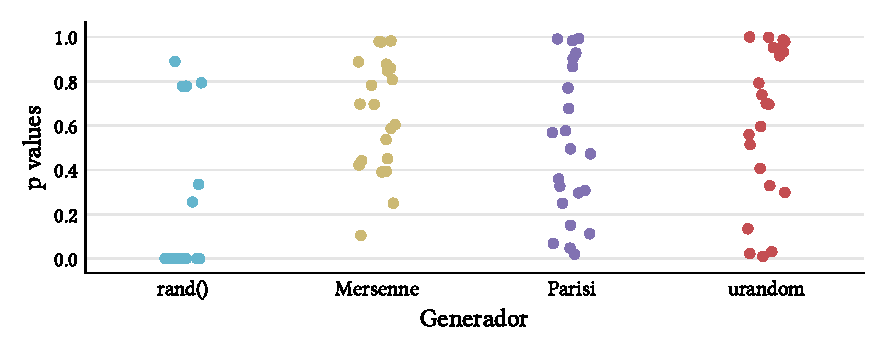
\includegraphics{../study_cases/dieharder/summary.pdf}
\end{center}



\chapter{Multispin coding}
\label{chap:multispin}

La simulación de vidrios de espín requiere un gran número de réplicas,
necesitándose correr varias simulaciones en paralelo. La naturaleza
binaria de los espines, que solo necesitan un bit para ser
codificados, hace que sea conveniente ``empaquetar'' varios en las
palabras de 32 o 64 bit de un ordenador en las iteraciones del
algoritmo de Metrópolis-Hasting~\cite{metropolis} empleado,
obteniendo paralelismo a nivel de bits como se verá a continuación.

Supongamos, para simplificar la explicación, un modelo de Ising simple
con hamiltoniano $\Ham = - \sum_{\expval{ij}}s_is_j$.
En cada iteración del algoritmo de Metrópolis-Hasting, necesitamos hallar
la energía de los espines y si es necesario voltearlos. Sin
optimizaciones, el algoritmo para actualizar cada espín sería el siguiente:
\begin{enumerate}
\item Calcular la energía con los 6 vecinos. Esto requiere una suma de
  6 términos $\sum_{j}s_j$, una multiplicación $s_i ⋅ \sum_{j}s_j$ y
  una negación por el signo menos del hamiltoniano.
\item Calcular la probabilidad $e^{-β \Ham_i}$ de volteo. La forma más
  eficiente de ejecutar este paso es construir una \textit{look up
    table} con los términos precalculados para los posibles valores de
  la energía $\Ham_i ∈ \{0,±4,±8,±12\}$, lo que además nos ahorra la
  negación aritmética anterior sin más que ordenar la tabla al revés.
\item Voltear el espín, si procede. Esto requiere una negación
  aritmética y el cálculo de un número aleatorio.
\end{enumerate}
Notar que en el algoritmo se han despreciado los accesos a la memoria
caché\footnote{Incluso para $L=40$, los datos necesarios (∼L³
  palabras de 64 bits para el código empleado) caben cómodamente en la
  memoria caché de Memento, el ordenador empleado.}.

La primera optimización que se puede realizar consiste en explotar el
carácter binario de los espines y emplear únicamente operaciones lógicas,
mucho más rápidas que las aritméticas. Para ello, pasamos de variables
$s∈\{±1\}$ a variables $σ∈\{0,1\}$. Vemos que $s=2σ+1$, por lo que
podemos traducir las sumas $\sum_{i}s_i$ a sumas en $σ$ con
facilidad. Además, las multiplicaciones se pueden sustituir por un
XOR y una negación asignando $+1→1$ y $-1→0$:
\begin{center}
  \begin{tabular}{cc|c}
    $s_1$ & $s_2$ & $s_1⋅s_2$ \\ \hline
    +1    & +1    &  +1 \\
    +1    & -1    &  -1 \\
    -1    & +1    &  -1 \\
    -1    & -1    &  +1 \\
  \end{tabular}
  \qquad
  \begin{tabular}{cc|c}
    $σ_1$ & $σ_2$ & $¬(σ_1⊕σ_2)$ \\ \hline
    1     & 1     & 1 \\
    1     & 0     & 0 \\
    0     & 1     & 0 \\
    0     & 0     & 1 \\
  \end{tabular}
\end{center}

Una vez que se ha pasado de operaciones aritméticas a lógicas se
puede explotar paralelismo en las propias palabras binarias
empleadas, en este caso de 64 bits. En cada palabra cabrían 64
espines, pero como la suma $\sum_{j}σ_j$ puede valer como máximo 6
(\texttt{110} en binario) necesitamos 3 bits por espín, de forma que caben 21
espines de diferentes sistemas por
palabra binaria\footnotemark:
\footnotetext{El bit sobrante ($21×3=63<64$) se ignora en el tratamiento
 y en el software.}


\begin{center}
  \begin{tabular}{l|c}
    Representación &                                                \\ \hline
    Espines        & \texttt{↑↑↓↑↓↑↓↓↓↓↓↓↑↓↑↑↓↑↓↑↑}                 \\
    Octal          & \texttt{110101000000101101011}                 \\
    Hexadecimal    & \texttt{1208200001048209}                      \\
    Binario        & \texttt{0.001.001.000.001.000.001.000}$\cdots$ \\
  \end{tabular}
\end{center}


Notar como al haber un espín por cada tres posiciones las posibles
palabras binarias en octal solo pueden tener los números 0 (000) o 1
(001); cualquier otra alternativa implicaría más de un espín por
posición. Por este motivo, la representación octal de las palabras
corresponde directamente a los espines, haciéndola especialmente útil
en la fase de \textit{debugging}.


El algoritmo mencionado previamente pasa a ser el siguiente:
\begin{enumerate}
\item Calculamos la energía con los vecinos. Para ello, comenzamos por
  hacer la suma $\sum_{j}σ_j$ de los seis primeros vecinos del espín $σ_i$:

  \begin{minipage}[lc]{1.0\linewidth}
    +
    \begin{tabular}{l}
     \texttt{0 000 001 000 000 001 001 000 000 000 000} \\
     \texttt{0 001 000 001 000 000 001 001 001 000 000} \\
     \texttt{0 001 001 000 001 001 000 000 001 000 001} \\
     \texttt{0 001 001 001 001 000 000 001 001 000 000} \\
     \texttt{0 000 000 000 000 001 001 000 001 000 001} \\
     \texttt{0 000 000 001 001 000 001 001 001 000 001} \\ \hline
     \texttt{0 011 011 011 011 011 100 011 101 000 011} \\
    \end{tabular}
  \end{minipage}

  donde se han truncado las palabras binarias a 31 bits por motivos de espacio.
  A continuación, multiplicamos por el $σ_i$ de
  $\Ham_i = σ_i \sum_{}σ_j$, donde $\sum_{}σ_j$ es la cantidad que
  acabamos de calcular. Para ello, hacemos un XOR lógico; no es
  necesario negarlo, ya que basta con alterar el orden de la
  \textit{look up table} en la que se guardan las probabilidades de la
  exponencial $e^{β\Ham_i}$.

  \begin{minipage}[lc]{1.0\linewidth}
    ⊕
    \begin{tabular}{l}
      \texttt{0 011 011 011 011 011 100 011 101 000 011} \\
      \texttt{0 001 001 000 001 001 000 001 001 000 000} \\ \hline
      \texttt{0 010 010 011 010 010 100 010 100 000 011} \\
    \end{tabular}
  \end{minipage}

\item Consultamos \emph{para cada uno de los 21 grupos de tres
    espines} el índice correspondiente en la \textit{look up table},
  obteniendo las 21 probabilidades $e^{-β \Ham}$. Con ellas,
  fabricamos una nueva palabra binaria de 64 bits que contiene 21 grupos de
  tres bits. Si el espín correspondiente se va a girar, se coloca
  \texttt{111}, si no \texttt{000}. Basta con hacer un XOR de $σ_i$
  con esta palabra binaria para girar los correspondientes espines.
\end{enumerate}

Hay que notar que el nuevo algoritmo necesita un bucle sobre los 21
espines de cada palabra, haciendo que a pesar de realizar operaciones
más simples (binarias frente a aritméticas) sea más lento. No
obstante, requiere 21 veces menos números aleatorios, y calcula en
paralelo la evolución de 21 sistemas, que en el caso de este trabajo
serán 21 muestras diferentes.

En los \textit{benchmarks} realizados se comprobó que este algoritmo
era tres veces más lento\footnote{Sin optimizaciones agresivas en el
  compilador (\texttt{-ffast-math -O2} en \texttt{clang} y
  \texttt{gcc}), es dos veces más lento.}, pero el gran aumento en
estadística que se tiene lo hace imprescindible: para sistemas de
$L<20$, son necesarias miles de muestras para obtener los valores
medios de algunos observables, como la correlación. Como referencia,
la simulación en un PC (Intel Core i7 cuarta generación) necesita
aproximadamente \SI{20}{\nano\second} por espín sin \textit{multispin
  coding} y \SI{60}{\nano\second} por cada grupo de 21 espines con él.

Cuando se simulan sistemas con $J$ variable hay que modificar
ligeramente el algoritmo~\cite{multispincoding}: en lugar de poder
sacar los acoplos $J_{ij}$ de la suma $\sum_{} J_{ij}σ_iσ_j$ como una
constante, es necesario multiplicarlos primero por los $σ_j$. Para
cada espín $σ_i$,
\begin{equation}
  \sum_{j} J_{ij} σ_i σ_j = σ_i \sum_{j} J_{ij} σ_j
\end{equation}

De forma que hay que realizar seis multiplicaciones $J_{ij}σ_j$ antes
de sumar los espines de los seis primeros vecinos y multiplicar por
$σ_i$. En el siguiente apéndice se muestra un ejemplo de implementación.

\chapter{Código fuente}
El código fuente de la memoria, incluyendo tanto la librería
desarrollada para las simulaciones como utilidades para realizarlas,
junto al código \LaTeX \ de la memoria y el empleado para generar las
gráficas, está disponible en un repositorio público de GitHub
en lugar de en un anexo por ser relativamente extenso:
\begin{flushright}
  \url{github.com/redpointyjackson/tfg}
\end{flushright}

El código para las simulaciones se ha escrito en C99, mientras que el
análisis de los datos se ha realizado en Julia~\cite{julialang} y Python.

A continuación se reproducen las dos funciones principales de la
librería principal, el cálculo de $\Ham_i = -\sum_{j} J_{ij} σ_i σ_j$
y el algoritmo de Metropolis-Hasting~\cite{metropolis}, en las que se
ve el uso de operaciones binarias para paralelizar la simulación
mediante \textit{multispin coding} (Apéndice~\ref{chap:multispin}).
Los $L^3$ espines se guardan en un vector unidimensional de palabras
binarias de 64 bits, y se emplean tablas precalculadas para calcular
la posición de los primeros vecinos (\texttt{guide\_left} y similares)
y las probabilidades $e^{β \Ham_i}$ (el campo \texttt{probs} dentro de
la estructura \texttt{SG}).

\vspace{1cm}

\begin{minted}{c}
uint64_t local_energy(struct net* SG, int64_t idx, int64_t x, int64_t y, int64_t z){
  uint64_t* S     = SG->spins;
  uint64_t* Jr    = SG->J_right;
  uint64_t* Ju    = SG->J_up;
  uint64_t* Jf    = SG->J_front;

  uint64_t right  = S[idx] ^ Jr[ idx                   ] ^ S[ idx + guide_right[x]  ];
  uint64_t left   = S[idx] ^ Jr[ idx + guide_left[x]   ] ^ S[ idx + guide_left[x]   ];
  uint64_t up     = S[idx] ^ Ju[ idx                   ] ^ S[ idx + guide_up[y]     ];
  uint64_t down   = S[idx] ^ Ju[ idx + guide_down[y]   ] ^ S[ idx + guide_down[y]   ];
  uint64_t front  = S[idx] ^ Jf[ idx                   ] ^ S[ idx + guide_front[z]  ];
  uint64_t behind = S[idx] ^ Jf[ idx + guide_behind[z] ] ^ S[ idx + guide_behind[z] ];

  return right + left + up + down + front + behind;
}
\end{minted}

\newpage

\begin{minted}{c}
void metropolis(struct net* SG){
  int64_t curr_idx = 0;
  int64_t L = SG->L;

  for(int64_t z=0;z<L;z++){
    for(int64_t y=0;y<L;y++){
      for(int64_t x=0;x<L;x++){

        uint64_t E = local_energy(SG, curr_idx, x, y, z);
        double randomnum = RANDOM_F;

        for(int_fast8_t spinidx=0; spinidx<21; spinidx++){

          uint64_t Pidx = E;
          Pidx = Pidx >> 3*spinidx;
          Pidx = Pidx &  0x7; // Select the first 3 bits.

          double P = SG->probs[Pidx];

          if (Pidx <= 3 || P > randomnum){
            uint64_t selectmask = 0x1;
            selectmask = selectmask << 3*spinidx;
            SG->spins[curr_idx] ^= selectmask; // Flip current σᵢ.
          }
        }
        curr_idx++;
      }
    }
  }
  SG->mc_steps++;
}
\end{minted}

\end{appendices}

\bibliography{biblio}

\vspace{1cm}

Silueta de la portada de \emph{Freepik} (\url{www.flaticon.com}).

\end{document}
